\begin{frame}{Aufgabe}
    \begin{center}
        https://github.com/tmwnd/adv\_cpp\_example.git
    \end{center}
\end{frame}

\begin{frame}[fragile]{pokemon.hpp}
    \begin{minted}{cpp}
struct Pokemon;     // id, name
struct Entwicklung; // pokemon_id

std::vector<Pokemon> get_pokemon();
std::map<int, Entwicklung> get_entwicklung();
    \end{minted}
\end{frame}

% \begin{frame}[fragile]{Pokemon}
%     \begin{minted}{cpp}
% struct Pokemon {
%     int id;
%     std::string name;
%     double groesse;
%     double gewicht;
%     int generation;
%     Typ primaer_typ;
%     Typ sekundaer_typ;
% };
%     \end{minted}
% \end{frame}

% \begin{frame}[fragile]{Entwicklung}
%     \begin{minted}{cpp}
% struct Entwicklung {
%     int pokemon_id;
%     int level;
%     int item_id;
%     int getragenes_item_id;
%     Tageszeit tageszeit;
% };
%     \end{minted}
% \end{frame}

\begin{frame}[fragile]{pokemon\_q.cpp}
    \begin{minted}{cpp}
auto pokemon = get_pokemon();
auto entwicklungen = get_entwicklung();
    \end{minted}
\end{frame}

\begin{frame}{Tipps}
    Schauen wir uns die gegebenen Daten an:

    \begin{center}
        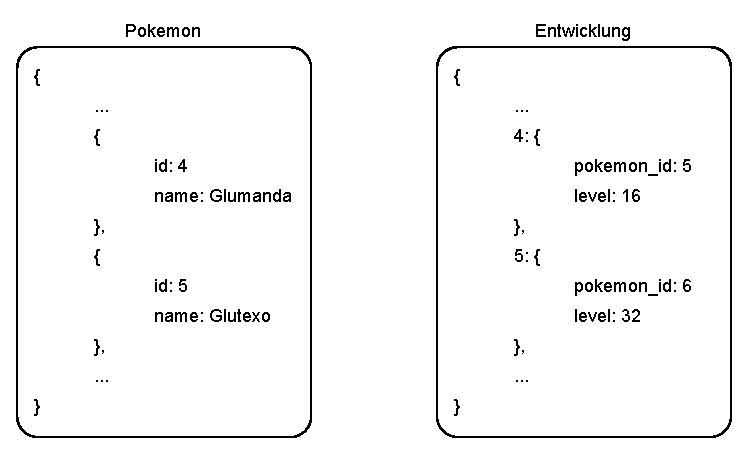
\includegraphics[width=0.75\textwidth]{pictures/example_1.pdf}
    \end{center}
\end{frame}

\begin{frame}{Tipps}
    Zuerst vergleichen wir die n-te \texttt{Pokemon.id} mit \texttt{Entwicklung.von}:

    \begin{center}
        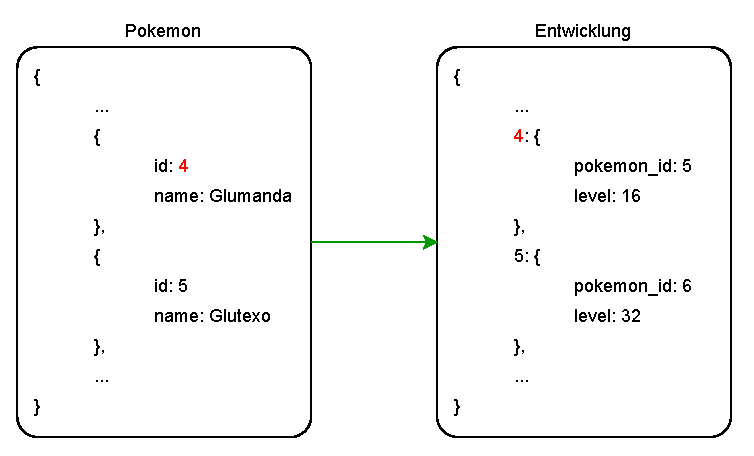
\includegraphics[width=0.75\textwidth]{pictures/example_2.pdf}
    \end{center}
\end{frame}

\begin{frame}{Tipps}
    Die erhaltene \texttt{Entwicklung.zu} finden wir in \texttt{Pokemon.id}:

    \begin{center}
        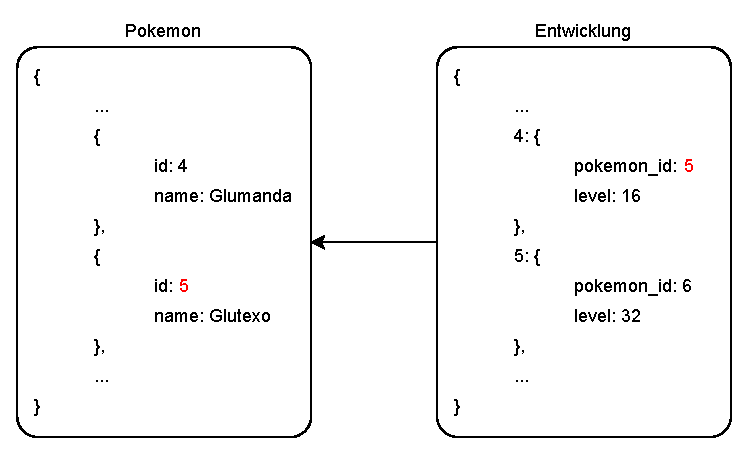
\includegraphics[width=0.75\textwidth]{pictures/example_3.pdf}
    \end{center}
\end{frame}

\begin{frame}{Tipps}
    Nun überschreiben wir das n-te Pokemon mit seiner Entwicklung:

    \begin{center}
        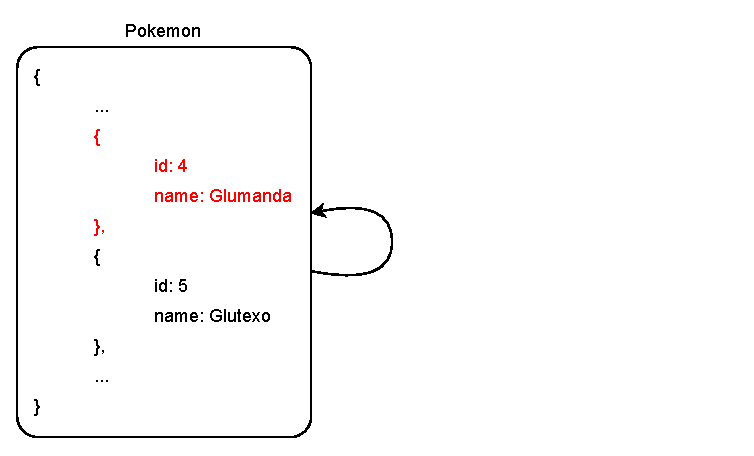
\includegraphics[width=0.75\textwidth]{pictures/example_4.pdf}
    \end{center}
\end{frame}

\begin{frame}{Tipps}
    Und erhalten:

    \begin{center}
        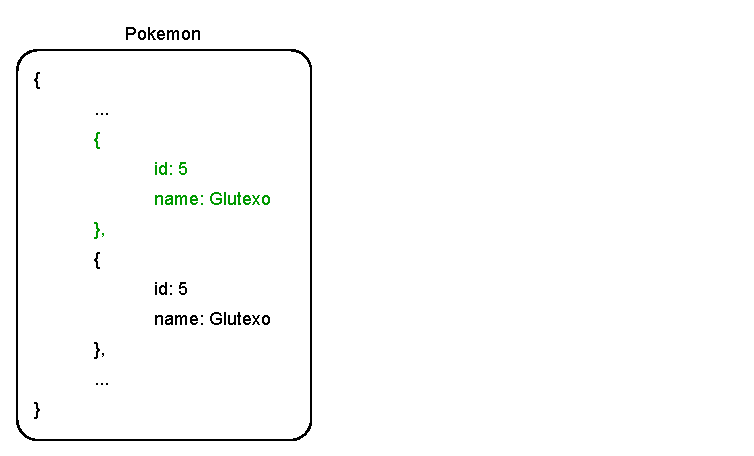
\includegraphics[width=0.75\textwidth]{pictures/example_5.pdf}
    \end{center}
\end{frame}

\begin{frame}{Tipps}
    Sollten wir das n-te Pokemon nicht finden:

    \begin{center}
        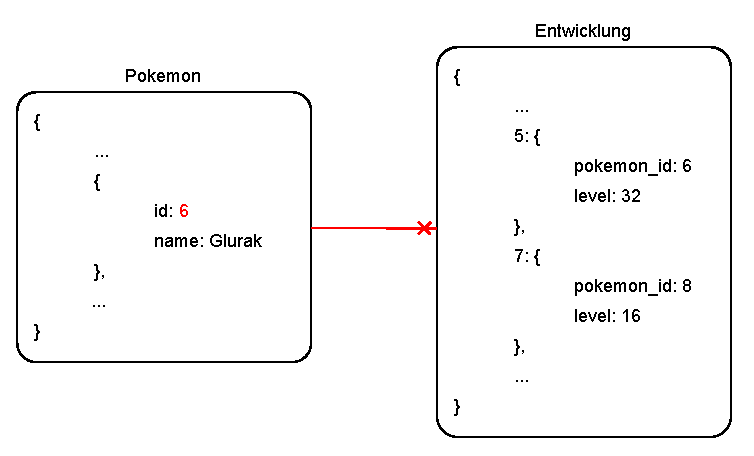
\includegraphics[width=0.75\textwidth]{pictures/example_6.pdf}
    \end{center}
\end{frame}

\begin{frame}{Tipps}
    entfernen wir dieses aus unserer View:

    \begin{center}
        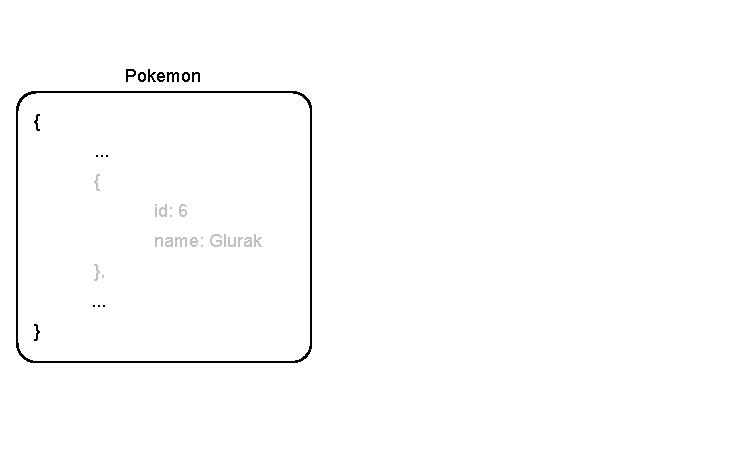
\includegraphics[width=0.75\textwidth]{pictures/example_7.pdf}
    \end{center}
\end{frame}